\newpage
\subsection{Resultados}
\label{subsection:resultados}
	tablas, gráficos, análisis y recomendaciones
	\begin{itemize}
		\item Aca debería explicar como fueron procesados los
                  resultados y que tipo de resultados se van a mostrar (ej. los
                  que tuvieron mejor y peor performance). \JS{hay que empezar a
                  poner cuales se van a mostrar y discutir}
                \item \JS{Baseline. Comparar con Wang}
		\item Resultados de dataset con imagenes reales.
		\begin{itemize}
			\item Se presentan los mejores resultados y los parámetros con los cuales se obtuvieron. Se van a presentar los gráficos de los 2 mejores resultados junto con sus matrices de confusión.
			\item Idem pero con los peores resultados obtenidos.
		\end{itemize}
		\item Idem con dataset sintéticos
		\item Idem con dataset sintéticos + reales.

	\end{itemize}
	
	Primero van a ir los resultados de Wang extraidos del paper y expuestos en una tabla. Se tiene que explicar que el resultado obtenido por Wang es el baseline para los experimentos realizados. Un vez que presente los mejores resultados obtenidos vuelvo a generar la tabla de comparacion.
	
	\begin{table}
		\centering
	    \begin{tabular}{ | l | l | l | p{5cm} |}
    			\hline
    				\textbf{Implementación} & \textbf{Score} \\ \hline
    				Wang NATIVE+FERNS & 0.54\% \\ \hline
    				Wang SINT+FERNS & 0.47\% \\
    			\hline
    		\end{tabular}	
    		\caption{Resultados obtenidos por Wang et al. en \cite{wang}}
	\end{table}

	Resultados de haber entrenado y evaluado al clasificador con imagenes reales. Básicamente busco mostrar que llegamos a resultados similares con Wang. Despues de mostrar los resultados, se puede agregar una tabla chiquita comparativa de los resultados.
	
			\begin{figure}[htbp!]
				\centering
				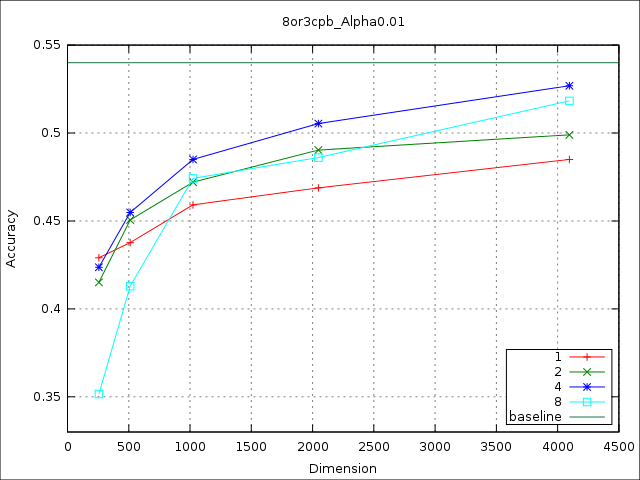
\includegraphics[scale=0.6]{img/resultados/reales/media_8or3cpb_Alpha0,01.png}
				\caption[Reales con umbral media]{Resultado de haber usado la media para la binarización de las características. La mejor clasificación se logra con los siguientes parámetros: \textit{alpha:0.01}, \textit{bits por grupo: 4}, \textit{dim del vector: 4096}, \textit{orientaciones: 8}, \textit{celdas por bloque: 9}.}
				\label{fig: Reales-media-8or9cpbAlph0.01}
			\end{figure}
			
			\begin{figure}[htbp]
				\centering
				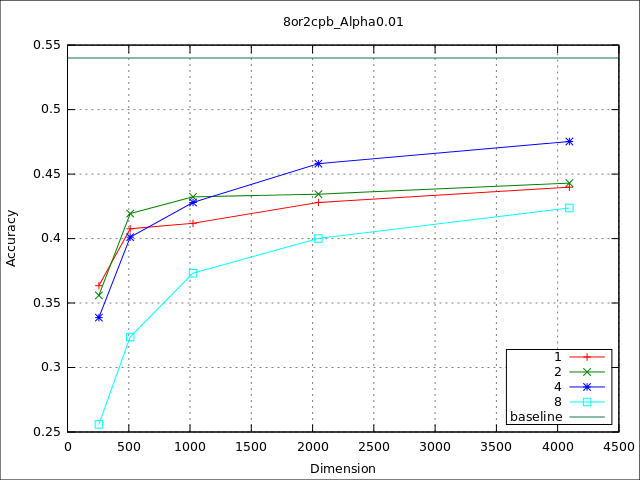
\includegraphics[scale=0.6]{img/resultados/reales/median_8or2cpb_Alpha0,01.png}
				\caption[Reales con umbral mediana]{Resultado de haber usado la mediana para la binarización de las características. La mejor clasificación se logra con los siguientes parámetros: \textit{alpha:0.01}, \textit{bits por grupo: 4}, \textit{dim del vector: 4096}, \textit{orientaciones: 8}, \textit{celdas por bloque: 4}.}
				\label{fig: Reales-mediana-8or4cpbAlph0.01}
			\end{figure}
			
			\begin{figure}[htbp]
				\centering
				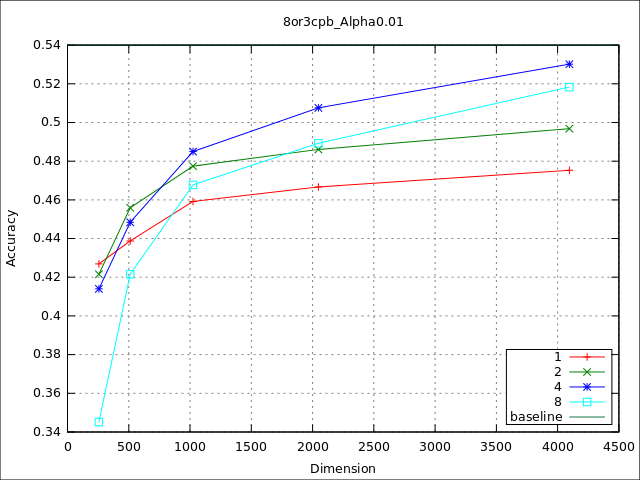
\includegraphics[scale=0.6]{img/resultados/reales/expon_8or3cpb_Alpha0,01.png}
				\caption[Reales con umbral exponencial]{Resultado de haber usado la distribución exponencial para la binarización de las características. La mejor clasificación se logra con los siguientes parámetros: \textit{alpha:0.01}, \textit{bits por grupo: 4}, \textit{dim del vector: 4096}, \textit{orientaciones: 8}, \textit{celdas por bloque: 9}.}
				\label{fig: Reales-expon-8or9cpbAlph0.01}
			\end{figure}
			
			\begin{figure}[htbp]
				\centering
				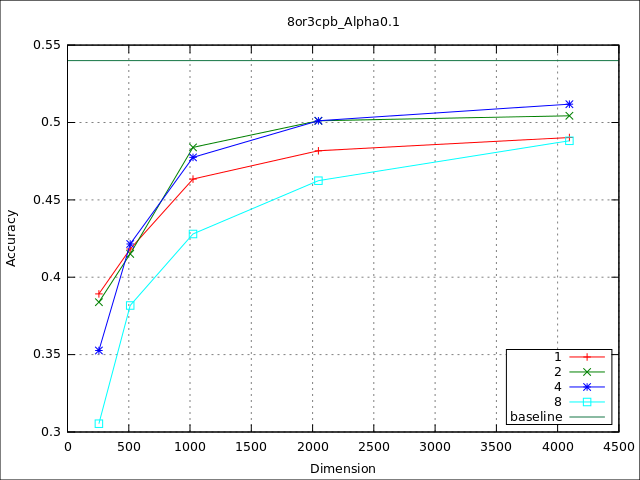
\includegraphics[scale=0.6]{img/resultados/reales/bootstrap_8or3cpb_Alpha0,1.png}
				\caption[Reales con umbral boostrap]{Resultado de haber usado bootstrap para la binarización de las características. La mejor clasificación se logra con los siguientes parámetros: \textit{alpha:0.1}, \textit{bits por grupo: 4}, \textit{dim del vector: 4096}, \textit{orientaciones: 8}, \textit{celdas por bloque: 9}.}
				\label{fig: Reales-bootstrap-8or9cpbAlph0.1}
			\end{figure}
			
		Después de presentar estos gráficos aclaro que los siguientes experimentos se realizaron utilizando la mejor configuración observada (8 orientaciones, 9 grupos por bloque). Comparación final con los resultados de Wang.
	\begin{table}
		\centering
		\begin{tabular}{ | l | l | l | p{5cm} |}
    			\hline
    				\textbf{NATIVE + FERNS} & \textbf{Score} \\ \hline
    				Wang et al. & 0.54\% \\ \hline
    				Media & 0.53\% \\ \hline
    				Mediana & 0.47\%\\ \hline
    				Exponencial & 0.53\% \\ \hline
    				Bootstrap & 0.51\%\\ 
    			\hline
    		\end{tabular}
    		\caption{Tabla comparativa entre el resultado obtenido por Wang para imágenes naturales y los obtenidos en el presente trabajo, utilizando los cuatro umbrales propuestos.}
    	\end{table}
    	
    	\newpage
    	Teniendo en cuenta el resultado de Wang para las imágenes sintéticas, paso a mostrar 
los resultados de haber ido incrementando la proporcion de muestras sintéticas al momento de entrenar al clasificador. Los siguientes gráficos representan la relación ``\textit{cantidad de imágenes sintéticas por clase}-\textit{precisión}''. Por cada método utilizado en la binarización se extrajeron dos imágenes. La primera representa la configuración de parámetros que devolvió el mejor resultado y la segunda el peor.

			\begin{figure}[htbp]
				\centering
				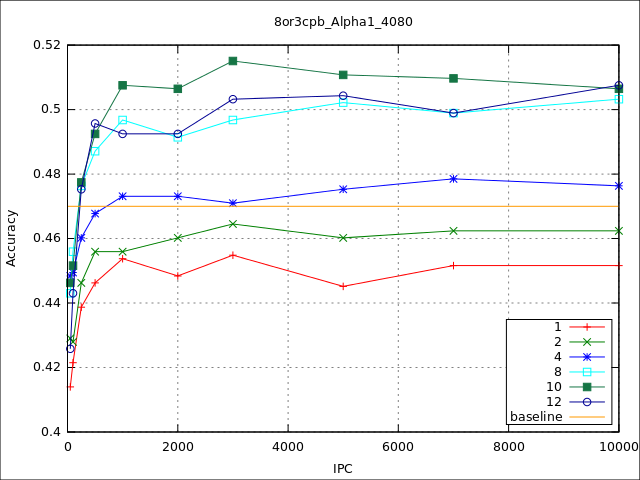
\includegraphics[scale=0.6]{img/resultados/sinteticas/best_media_8or3cpb_Alpha1_4080.png}
				\caption[Sintéticas media mejor resultado]{El gráfico muestra la configuración que devolvió los mejores resultados al utilizar la media en la binarización.}
				\label{fig: Sinteticas-media-mejor}
			\end{figure}
			
			\begin{figure}[htbp]
				\centering
				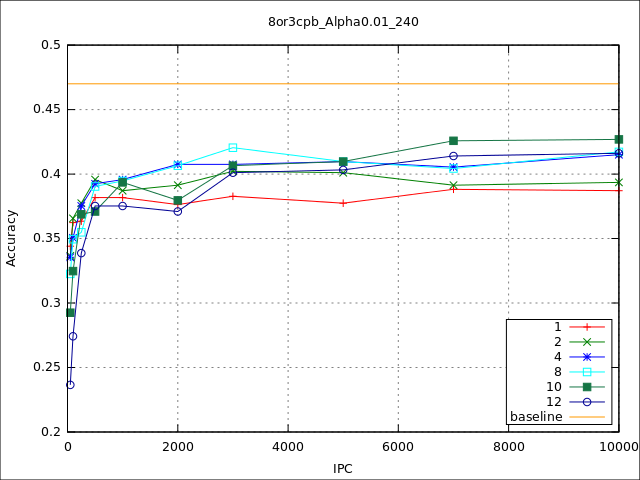
\includegraphics[scale=0.6]{img/resultados/sinteticas/worst_media_8or3cpb_Alpha0,01_240.png}
				\caption[Sintéticas media bajo resultado]{El gráfico muestra la configuración que devolvió los peores resultados al utilizar la media en la binarización.}
				\label{fig: Sinteticas-media-bajo}
			\end{figure}
			
			\begin{figure}[htbp]
				\centering
				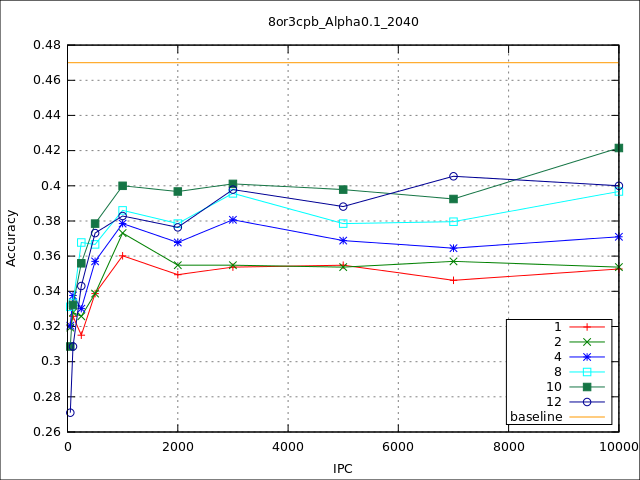
\includegraphics[scale=0.6]{img/resultados/sinteticas/best_median_8or3cpb_Alpha0,1_2040.png}
				\caption[Sintéticas mediana mejor resultado]{El gráfico muestra la configuración que devolvió los mejores resultados al utilizar la mediana en la binarización.}
				\label{fig: Sinteticas-median-mejor}
			\end{figure}
	
			\begin{figure}[htbp]
				\centering
				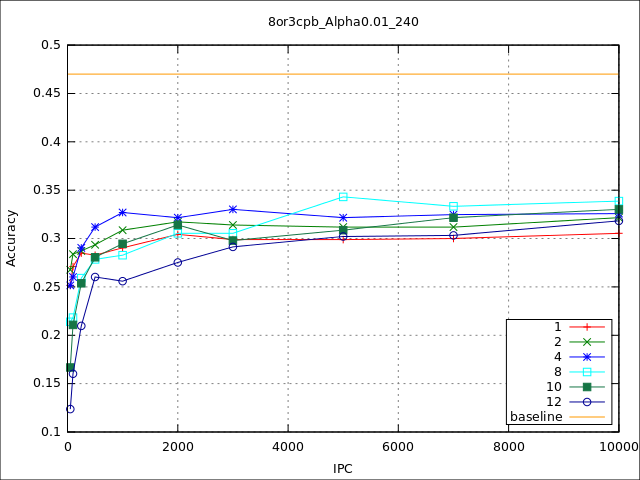
\includegraphics[scale=0.6]{img/resultados/sinteticas/worst_median_8or3cpb_Alpha0,01_240.png}
				\caption[Sintéticas mediana peor resultado]{El gráfico muestra la configuración que devolvió los peores resultados al utilizar la mediana en la binarización.}
				\label{fig: Sinteticas-median-bajo}
			\end{figure}
				
			\begin{figure}[htbp]
				\centering
				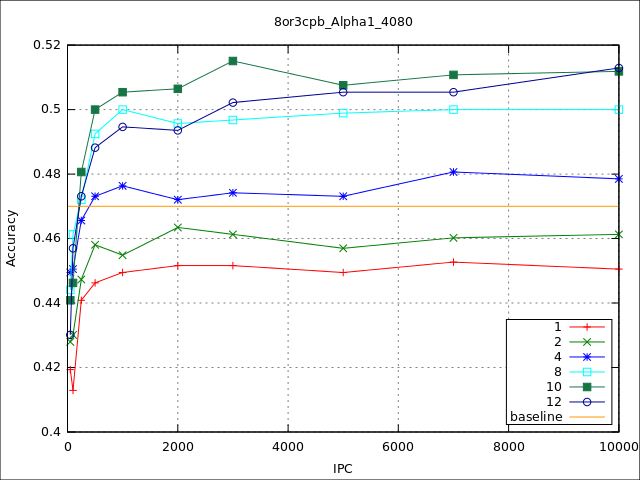
\includegraphics[scale=0.6]{img/resultados/sinteticas/best_expon_8or3cpb_Alpha1_4080.png}
				\caption[Sintéticas exponencial mejor resultado]{El gráfico muestra la configuración que devolvió los mejores resultados al utilizar la distribución exponencial en la binarización.}
				\label{fig: Sinteticas-expon-mejor}
			\end{figure}
	
			\begin{figure}[htbp]
				\centering
				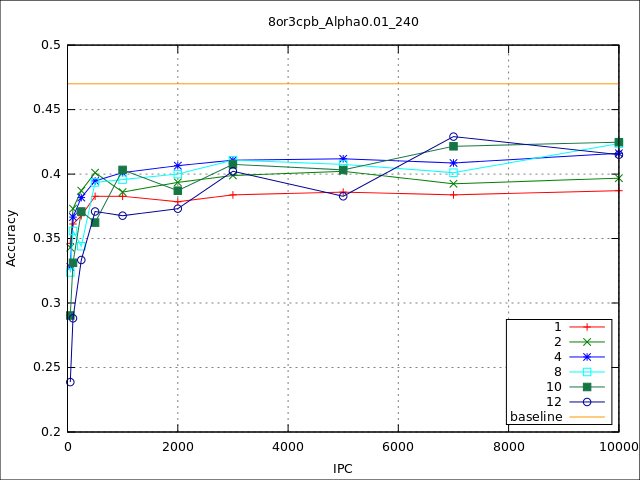
\includegraphics[scale=0.6]{img/resultados/sinteticas/worst_expon_8or3cpb_Alpha0,01_240.png}
				\caption[Sintéticas exponencial peor resultado]{El gráfico muestra la configuración que devolvió los peores resultados al utilizar la distribución exponencial en la binarización.}
				\label{fig: Sinteticas-expon-bajo}
			\end{figure}
			
			\begin{figure}[htbp]
				\centering
				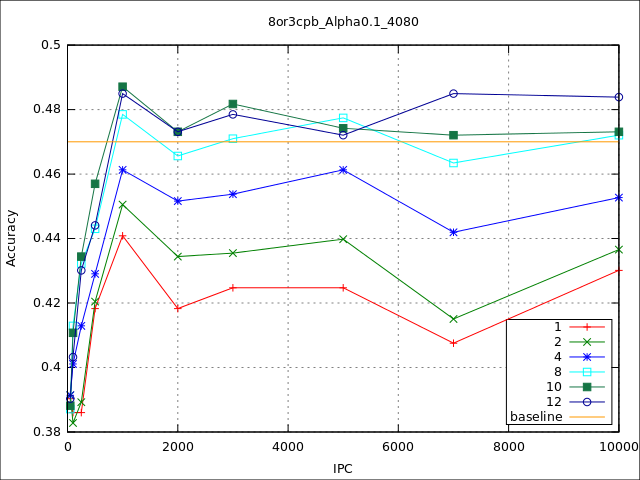
\includegraphics[scale=0.6]{img/resultados/sinteticas/best_bootstrap_8or3cpb_Alpha0,1_4080.png}
				\caption[Sintéticas bootstrap mejor resultado]{El gráfico muestra la configuración que devolvió los mejores resultados al utilizar bootstrap en la binarización.}
				\label{fig: Sinteticas-bootstrap-mejor}
			\end{figure}
	
			\begin{figure}[htbp]
				\centering
				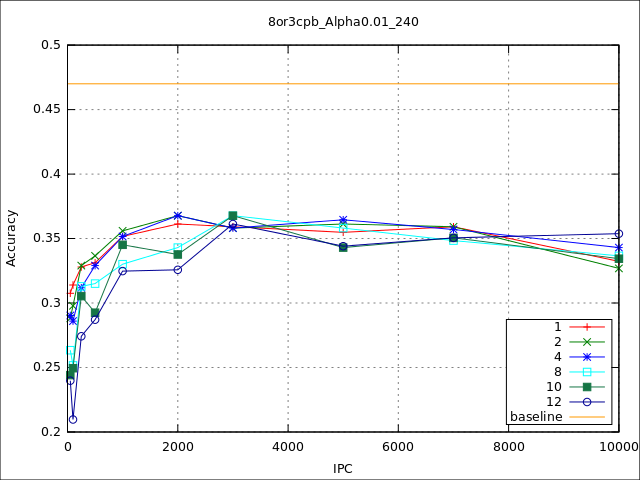
\includegraphics[scale=0.6]{img/resultados/sinteticas/worst_bootstrap_8or3cpb_Alpha0,01_240.png}
				\caption[Sintéticas bootstrap peor resultado]{El gráfico muestra la configuración que devolvió los peores resultados al utilizar bootstrap en la binarización.}
				\label{fig: Sinteticas-bootstrap-bajo}
			\end{figure}


	\begin{table}
		\centering
		\begin{tabular}{ | l | l | l | p{5cm} |}
    			\hline
    				\textbf{SINT(1000) + FERNS} & \textbf{Score} \\ \hline
    				Wang et al. & 0.47\% \\ \hline
    				Media & 0.51\% \\ \hline
    				Mediana & 0.4\%\\ \hline
    				Exponencial & 0.5\% \\ \hline
    				Bootstrap & 0.49\%\\ 
    			\hline
    		\end{tabular}
    		\caption{Tabla comparativa entre el resultado obtenido por Wang para imágenes sintéticas y los obtenidos en el presente trabajo, utilizando los mejores resultados entre los cuatro umbrales propuestos. Se consideran para poder realizar la comparación los resultados cuando se evalua al clasificador con 1000 imágenes sintéticas.}
    	\end{table}
			
\newpage
	Por último se van a mostrar los resultados correspondientes de haber entrenado al clasificador con conjuntos de entrenamiento mixtos. Se procederá a mostrar los gráficos con las mejores y peores configuraciones y sus resultados. También se mostrarán las matrices de correlación para todos estos casos. Teniendo en cuenta los resultados anteriores, se van a mostrar los resultados de haber utilizado solamente la distribución exponencial como umbral ya que fue la que obtuvo los mejores resultados. En los gráficos  se van a mostrar también los baselines de Wang et al. para las imágenes reales y las sintéticas.
	
			\begin{figure}[htbp]
				\centering
				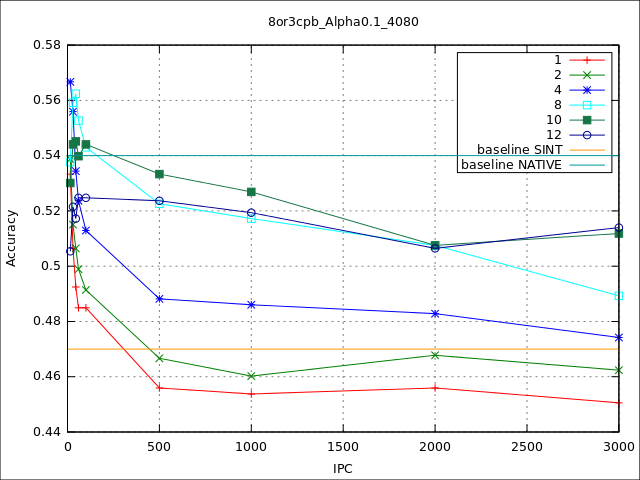
\includegraphics[scale=0.6]{img/resultados/mixtas/best_expon_8or3cpb_Alpha0,1_4080.png}
				\caption[Mixtas expon mejor resultado]{El gráfico muestra la configuración que devolvió los mejores resultados.}
				\label{fig: Mixtas-expon-mejor}
			\end{figure}

			\begin{figure}[!htbp]
				\centerline{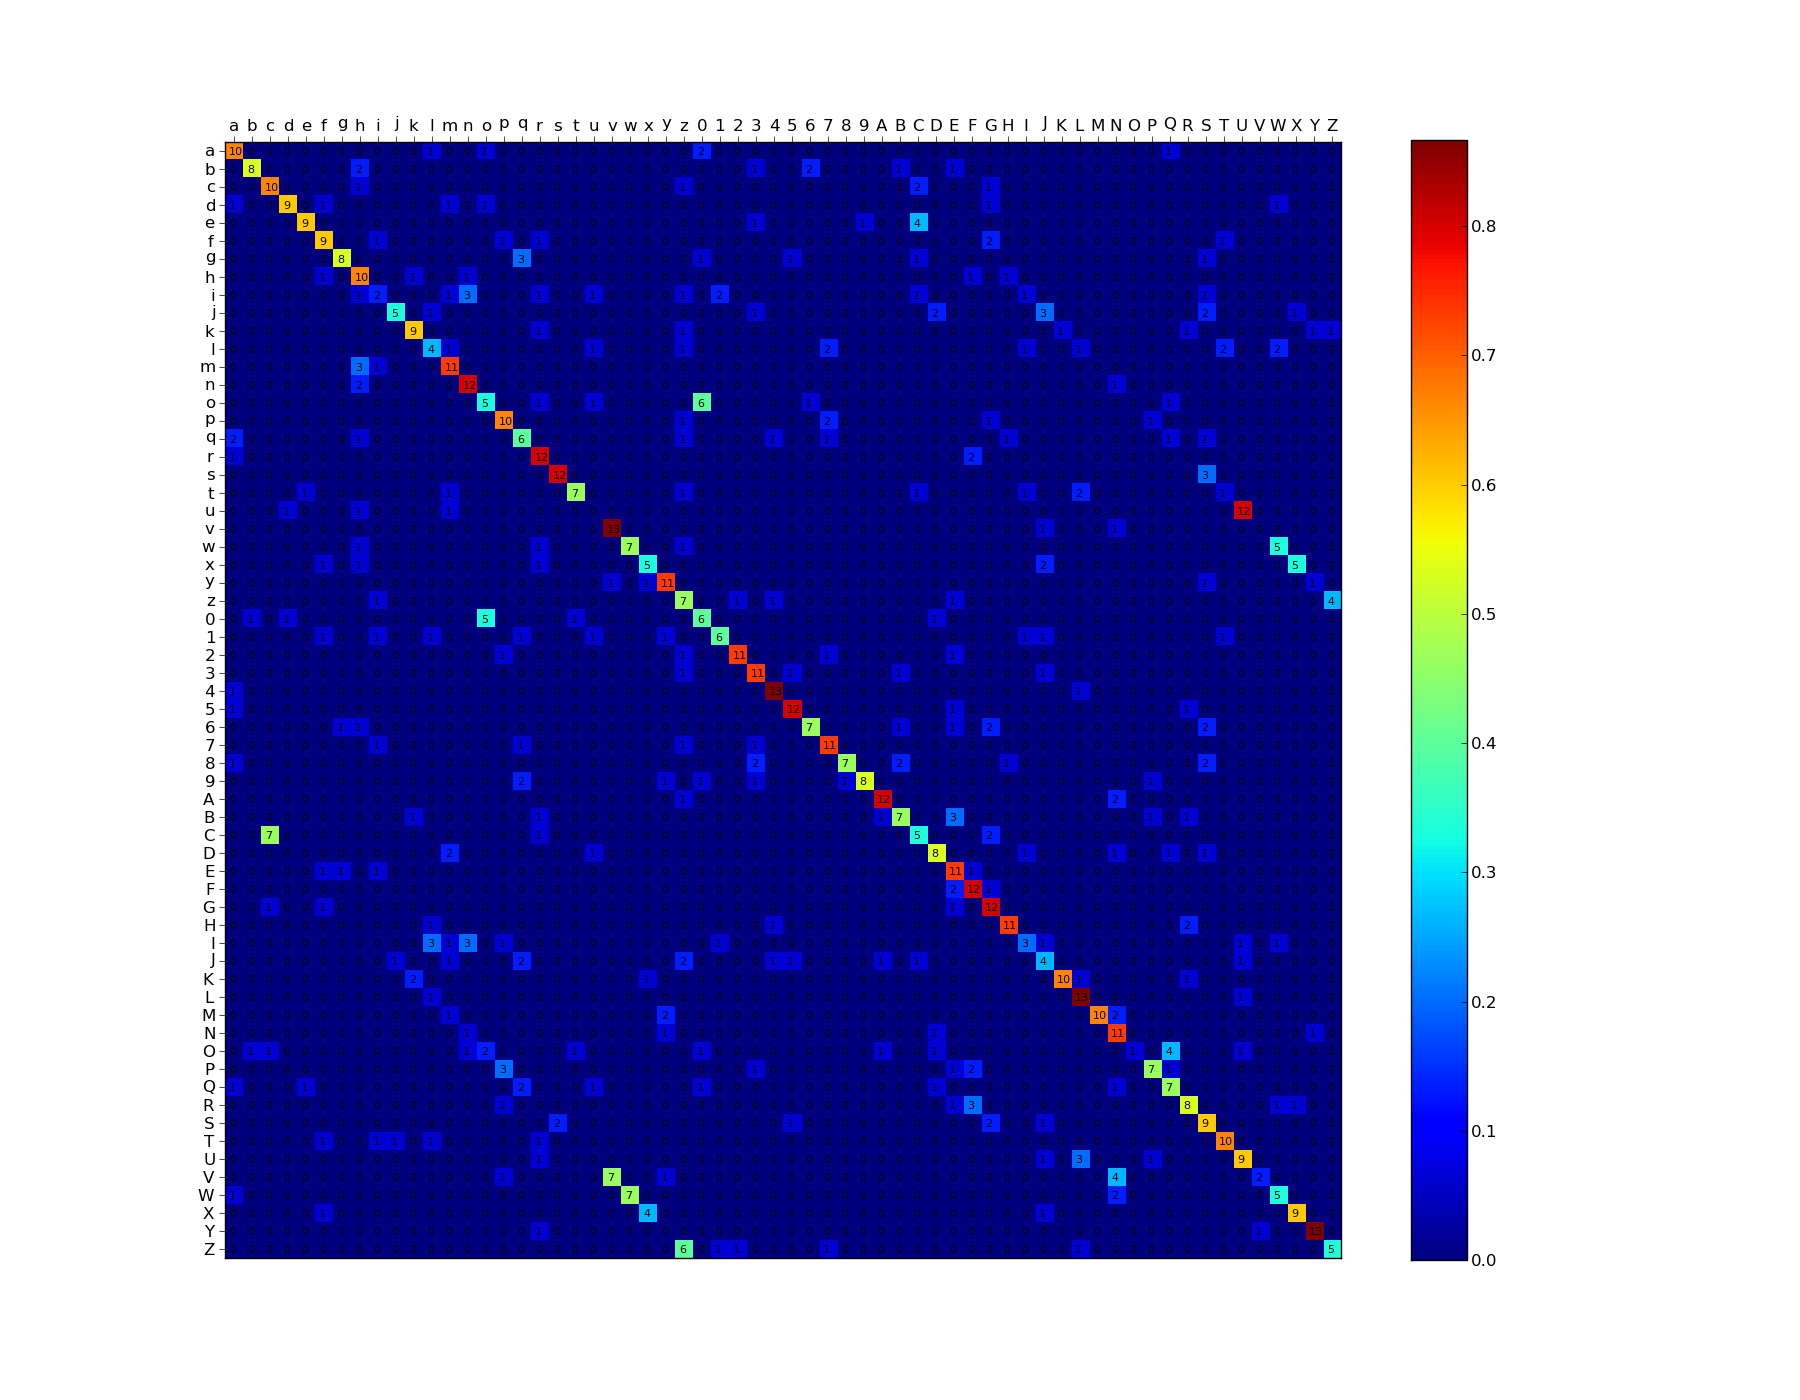
\includegraphics[scale=0.4]{img/resultados/mixtas/best_expon_matrix_Alpha0,1_4080-4.png}}
				\caption[Mixtas Matriz expon]{Matriz de correlación del gráfico \ref{fig: Mixtas-expon-mejor} para el mejor resultado. \RC{Demasiado grande las matrices como para mostrarlas y que se vean bien}}
				\label{fig: Mixtas-Matrix-expon-mejor}
			\end{figure}
	
			\begin{figure}[htbp]
				\centerline{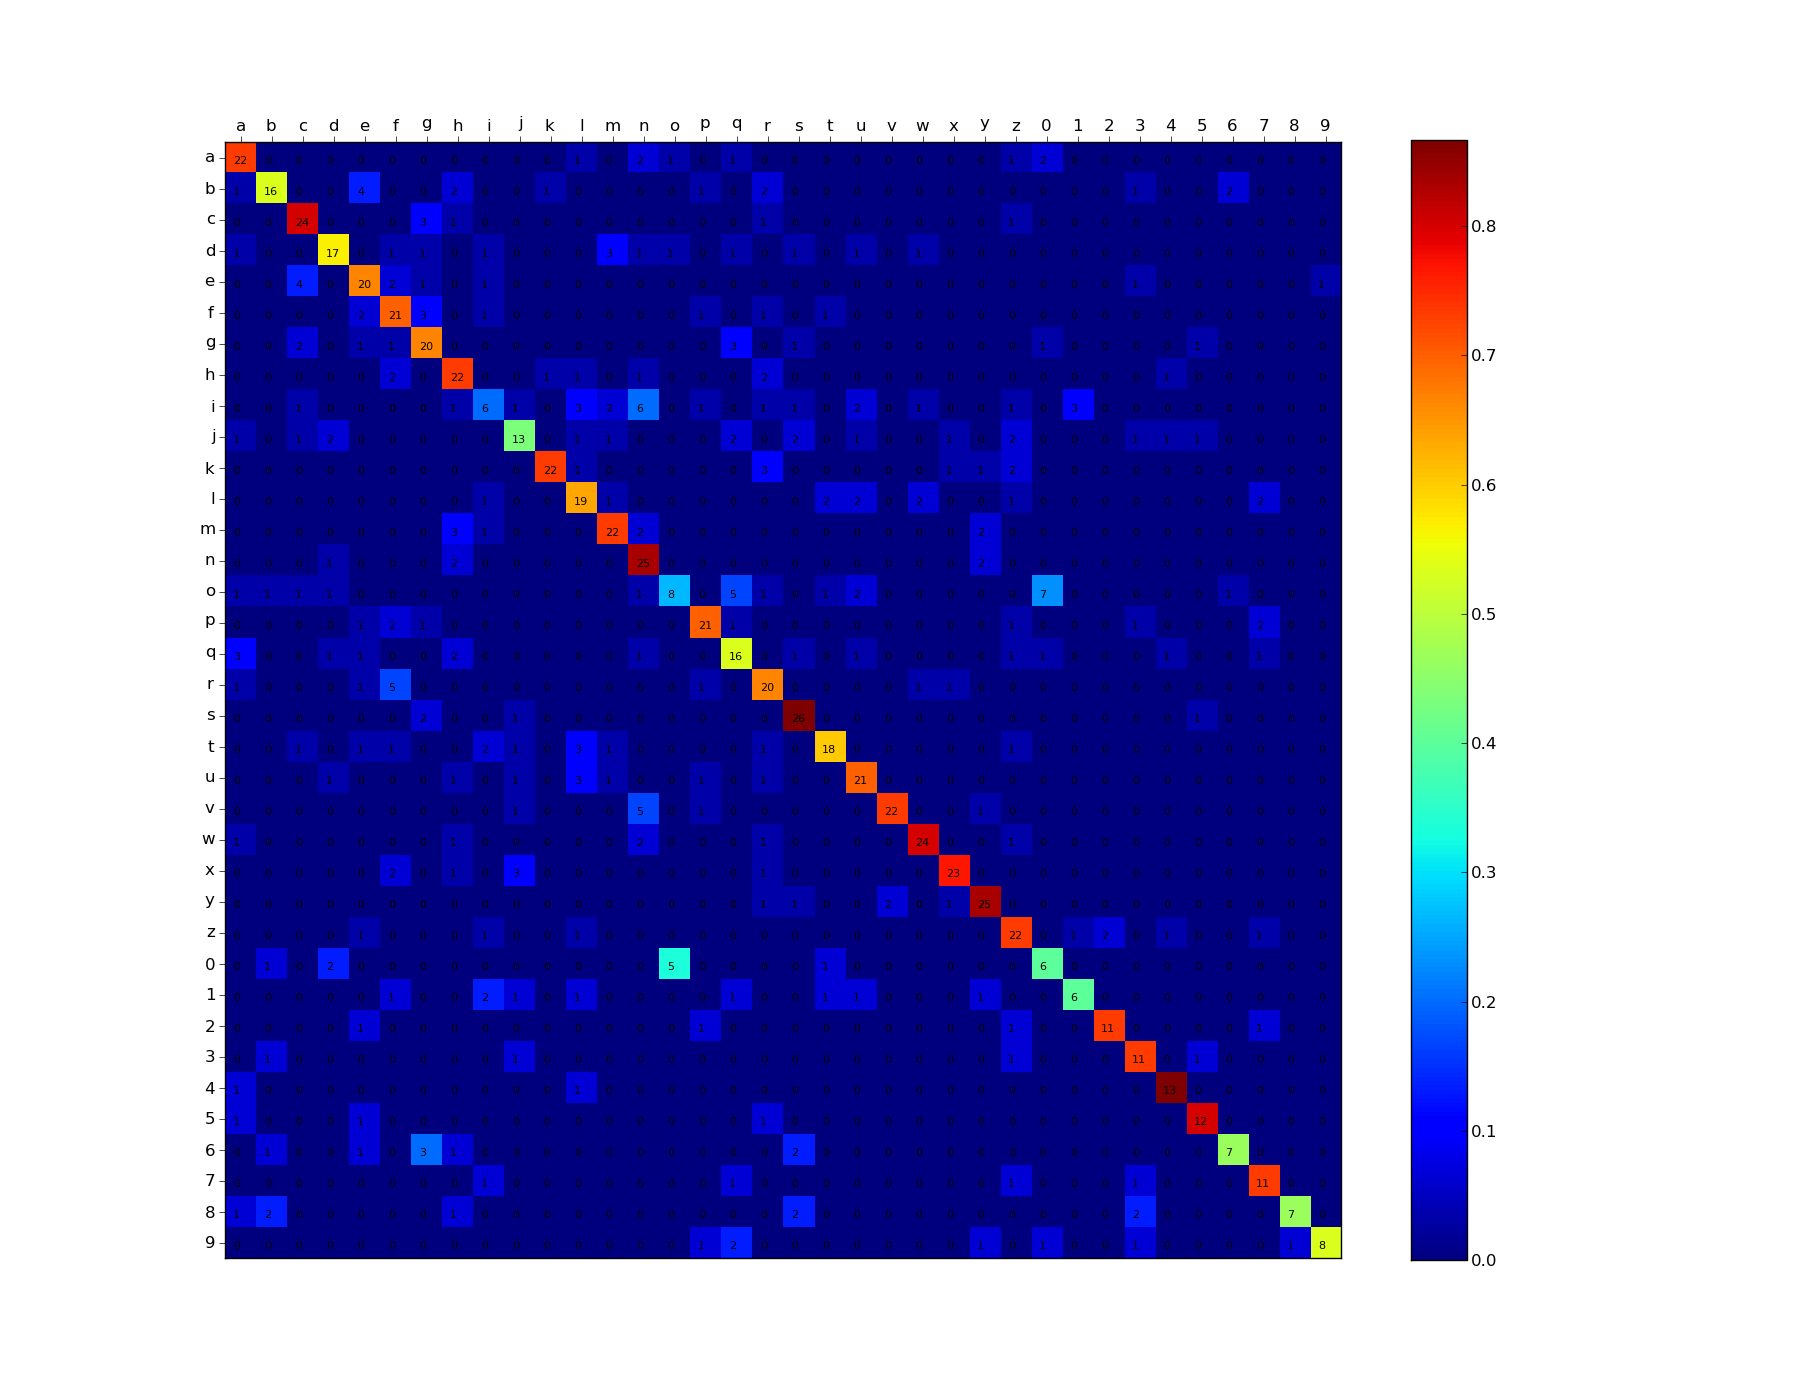
\includegraphics[scale=0.4]{img/resultados/mixtas/best_expon_matrix_Alpha0,1_4080-4_ins.png}}
				\caption[Matriz de correlación ``case insensitive'' para mixtas expon]{Matriz de correlación del gráfico \ref{fig: Mixtas-expon-mejor} para el mejor resultado no teniendo en cuenta los caracteres en mayúscula.}
				\label{fig: MatrizIns-Mixtas-expon}
			\end{figure}